\apendice{Documentación técnica de programación}

\section{Introducción}
En este apéndice se explicarán todos los aspectos relevantes del proyecto con el objetivo de facilitar la comprensión del mismo si otro desarrollador quisiera continuar con el trabajo o entenderlo más a fondo.

\section{Estructura de directorios}

El proyecto está alojado en dos repositorios diferentes. El motivo, es el de conseguir un despliegue automático a través de la plataforma \emph{heroku}. Por lo que nos encontramos con:

\subsection{Web Jellyfish Forecast}
Es el repositorio\footnote{Web Jellyfish Forecast. \url{https://github.com/psnti/WebJellyfishForecast}} en el que se alojan todos los ficheros necesarios para el funcionamiento de la aplicación web.

Contiene los siguientes directorios:
\begin{itemize}
	\item \textbf{Documentos}: Se guardan, el dataframe en el que estan la relación de playas con sus coordenadas así como un fichero excel con los avistamientos, necesario para realizar el historial de avistamientos.
	\item \textbf{static}: Aloja los ficheros css y javascript así como las imágenes necesarios para el buen funcionamiento de la aplicación.
	\item \textbf{templates}: Contiene los ficheros html.
\end{itemize}

Tambien contiene los siguientes archivos:
\begin{itemize}
	\item \textbf{Procfile}: Archivo necesario para el despliegue en \emph{Heroku} que contiene el comando que debe ejecutar la app en el arranque.
	\item \textbf{app.py}: Archivo python con la funcionalidad de la aplicación.
	\item \textbf{requirements.txt}: Listado de bibliotecas que se deben instalar en la máquina antes de ejecutar la aplicación.
\end{itemize}

\subsection{Jellyfish Forecast}
Es el repositorio\footnote{Jellyfish Forecast. \url{https://github.com/psnti/Jellyfish_Forecast}} en el que se alojan el resto de archivos del proyecto.

Contiene los siguientes directorios:
\begin{itemize}
	\item \textbf{Web}: Contiene el boceto de la aplicación realizado antes del desarrollo de la misma asi como una referencia al anterior repositorio.
	\item \textbf{docs/latex}: Aloja la documentación del proyecto.
	\item \textbf{src}: Contiene todo el código utilizado para la descarga y tratamiento de los datos así como el entrenamiento del modelo.
\end{itemize}

\section{Manual del programador}

Este apartado está destinado a la explicación de la instalación de todo lo necesario para poder ejecutar el proyecto o programadores que quieran trabajar en la mejora del mismo.

Para la ejecución del proyecto es indispensable la instalación de Python (el desarrollo se ha realizado con la versión 3.7.6). Posteriormente se instalarán los paquetes recogidos en el fichero requirements.txt como se indica en el apartado \ref{D4}.

En cuanto a la generación del modelo la mayoría del código está elaborado con \emph{jupyter notebook} por lo que es necesaria su instalación. La manera más sencilla es instalando \emph{Anaconda}\footnote{Anaconda. \url{https://www.anaconda.com/products/individual}}.

\section{Compilación, instalación y ejecución del proyecto}\label{D4}

En este apartado se indicará el proceso de obtener proyecto desde el repositorio hasta su despliegue en la plataforma de \emph{Heroku}.

\subsection{Descargar el proyecto}\label{Descarga}

\begin{enumerate}
	\item En primer lugar se ha de acceder al repositorio\footnote{Web Jellyfish Forecast. \url{https://github.com/psnti/WebJellyfishForecast}}.
	\item Descargar el contenido desde \textbf{Clone or Download}
	\imagen{clone_download.png}{Descargar repositorio}\label{clone}
	\item Descomprimir el fichero .zip en la ruta deseada.
	\item Antes de instalar las bibliotecas utilizadas en el proyecto crearemos un entorno virtual y accederemos a el:
	\begin{verbatim}
	Python -m venv env
	env\Scripts\active.bat
	\end{verbatim}
	\item Para la instalación de la biblioteca necesarias, contamos con el archivo requirements.txt. Ejecutando el siguiente comando, se instalarán todas las dependencias del proyecto en  nuestro entorno virtual.
	\begin{verbatim}
	pip install -r requirements.txt
	\end{verbatim}
	
\end{enumerate}

\subsection{Ejecutar aplicación}

\begin{enumerate}
	\item Una vez instaladas todas las dependencias, podremos ejecutar la aplicación. Desde el entorno virtual ejecutamos:
	\begin{verbatim}
	Flask run
	\end{verbatim}
	\item Accederemos desde el navegador a la dirección \href{http://127.0.0.1:5000}{http://127.0.0.1:5000}
	
\end{enumerate}

\subsection{Modificación de los datos}

Si se quisiera modificar el listado de playas que aparecen en la aplicación se deberá editar o sustituir el fichero ``listado\_playas.pkl'' contenido en el directorio ``documentos'' donde se recogen el nombre la playa con sus respectivas coordenadas. En este mismo directorio se encuentra el documento excel con los avistamientos de las medusas (``Datos\_Physalia\_20171010.xls'') y del que se extraen los datos para generar el gráfico del historial de cada playa. 

Si se modifica el fichero con el listado de las playas, los nombres de las mismas deberán coincidir con los que aparecen en el archivo excel si se quiere que el gráfico del historial tenga contenido.

En cuanto al modelo predictivo, se encuentra en la carpeta ``static''.

\subsection{Despliegue de la aplicación}

El despliegue se realizó en la plataforma \emph{Heroku} pues es gratuita y los recursos que ofrece son suficientes para los requisitos de nuestro proyecto.

Hay dos ficheros importantes para el despliegue:
\begin{itemize}
	\item \textbf{requirements.txt}: como se ha mencionado anteriormente, recoge todas las dependencias del proyecto y es necesario para que se instalen en la maquina antes de ejecutarlo. Si se añaden bibliotecas se deberá reflejar en este archivo. Dentro del entorno virtual ejecutaremos:
	\begin{verbatim}
	pip freeze > requirements.txt
	\end{verbatim}
	De esta manera se actualizarán todas la bibliotecas instaladas en el entorno virtual.
	\item En segundo lugar, el archivo \textbf{Procfile}. Contiene el comando que debe ejecutar la app en el arranque y debe ir sin extensión.
\end{itemize}


Una vez tengamos estos archivos deberemos seguir los siguientes pasos:
\begin{enumerate}
	\item Acceder a la pagina de \emph{Heroku}\footnote{Heroku \url{https://www.heroku.com/}} y crear una cuenta.
	\item Entraremos en nuestra cuenta, y en el panel de usuario crearemos una nueva \emph{app}.
	\begin{figure}[!h]
		\centering
		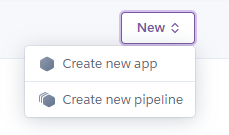
\includegraphics[width=0.6\textwidth]{new_app.png}
		\caption{Nueva app en \emph{Heroku}}\label{fig:new_app}
	\end{figure}
	\item Añadimos un nombre para nuestra aplicación y ya tendremos nuestra app creada.
	\begin{figure}[!h]
		\centering
		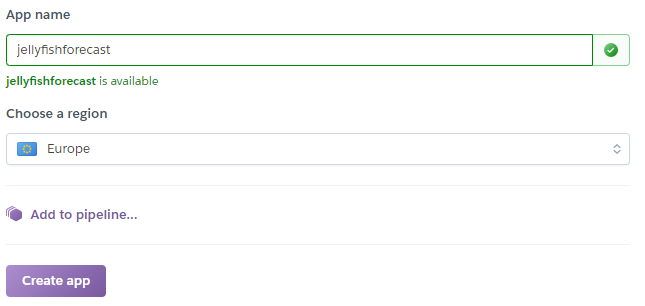
\includegraphics[width=0.9\textwidth]{nombre_app.png}
		\caption{Nombrar nueva app en \emph{Heroku}}\label{fig:new_app}
	\end{figure}
	\item A la hora de realizar el despliegue tendremos dos opciones: asociar la aplicación a un repositorio existente de \emph{GitHub}, o crear un nuevo repositorio en \emph{Heroku}. En el caso de este proyecto se eligió la opción de asociarlo a un repositorio en \emph{GitHub}. 
	
	Si se prefiriese el repositorio en \emph{Heroku} las instrucciones para su creación aparecen en la pagina de la aplicación.
	\begin{figure}[!h]
		\centering
		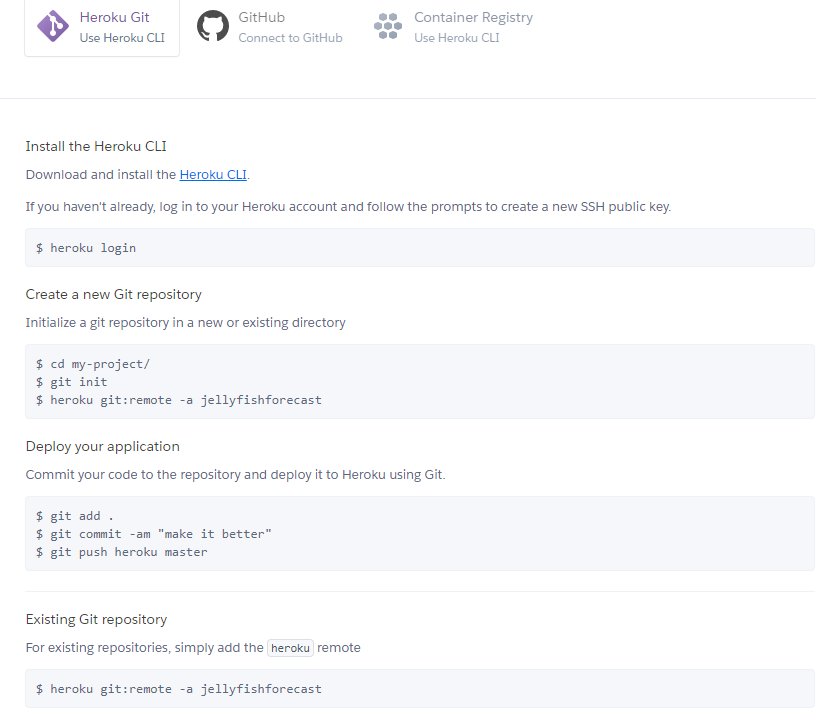
\includegraphics[width=0.9\textwidth]{deploy_heroku.png}
		\caption{Modos de despliegue en \emph{Heroku}}\label{fig:deploy}
	\end{figure}
		
\end{enumerate}

\subsection{Generación del modelo}

La generación del modelo y las pruebas están recogidas en el segundo repositorio\footnote{Jellyfish Forecast. \url{https://github.com/psnti/Jellyfish_Forecast}}. La forma de descargarlo e instalar todas las bibliotecas necesarias es igual a lo explicado en el anterior repositorio.

En la carpeta ``scr/Descarga datos'' podremos encontrar dos scripts diferentes para poder descargar los datos oceánicos de origen desde \emph{Copernicus}. Uno lo hace a través de una API. Esta opción se descartó, pues en el momento de descargar los datos era bastante nueva y originaba errores, además de tardar demasiado en generar los paquetes de datos. El otro, descarga los datos a través de un FTP. Esta opción descarga un volumen mucho mayor pues se descargan los datos de cada día y de todo el mundo, por lo que tras descargar cada archivo, el script realiza un \emph{crop} dejando unicamente el área de Chile y las variables que nos interesan para el estudio como se explica en el apartado \ref{diseño_datos}

Si nos movemos a la carpeta ``src/Avistamientos'' nos encontramos con los \emph{notebooks} utilizados para la generación del modelo predictivo.
\begin{itemize}
	\item En la carpeta ``\textbf{\#ExcelsAvistamientosIniciales}'' encontraremos los conjuntos de datos de los avistamientos. La versión más reciente es ``Datos\_Physalia\_20171010.xls''.
	\item El archivo GenerarEstructura.ipynb realiza todo el trabajo de tratar los conjuntos de datos, unirles y generar una estructura que posteriormente se utilizará para entrenar al modelo. Estas estructuras se guardan en dos formatos distintos. En la carpeta ``Excels'' están los archivos con formato .xlsx para consulta, pues son más fáciles de visualizar. Por otro lado, en la carpeta ``pkls'' se encuentran los archivos con formato .pkl que son con los que se trabaja pues su lectura y guardado son más eficientes de leer y guardar.
	\item La carpeta ``PruebasGeneracionEstructuraDatos'' contiene varios \emph{notebooks} con pruebas de las diferentes transformaciones que se han realizado a la estructura de datos. 
	\item Por ultimo, ``GeneracionModelo'' contiene algunas pruebas que se realizaron a la hora del aprendizaje con \emph{Scikit-learn} y tres \emph{notebooks} con las  pruebas realizadas con diferentes algoritmos.
\end{itemize}

\section{Pruebas del sistema}

\subsection{Pruebas de funcionamiento}
A parte de las pruebas por parte de los usuarios, se han realizado pruebas automáticas utilizando la herramienta \emph{Selenium}.

Se ha utilizado la biblioteca para Python con el driver correspondiente para Google Chrome. Elegí esta opción en vez de utilizar la extensión disponible debido a tener una breve experiencia con esta biblioteca. 

La versión de Chrome con la que se ha utilizado ha sido la 83.0.4103.106 con el driver correspondiente para esta versión. Si se prueba en el futuro, es probable que la versión del navegador sea diferente. Habría que descargar la versión correspondiente del driver\footnote{Web para descarga del ChromeDriver. \url{https://chromedriver.chromium.org/downloads}}, e introducirla en la carpeta ``test/chromedriver'' del repositorio \emph{WebJellyfishForecast}.

Para ejecutar las pruebas, accederemos el entorno virtual como se ha explicado en el punto anterior y ejecutaremos el fichero \emph{test.py}.
\begin{verbatim}
Python test/test.py
\end{verbatim}

Esta ejecución genera un fichero ``test.log'' con las salida de los test.

También se han realizado pruebas del correcto funcionamiento de la aplicación en diferentes navegadores web. Google Chrome, Firefox y Opera soportan toda las funcionalidad de la aplicación, mientras que en Microsoft Edge no se cargan los mapas.\label{pruebas_navegadores}

\subsection{Pruebas del modelo}

Además de las pruebas de la aplicación web, se realizan pruebas comparativas entre diferentes algoritmos de aprendizaje sobre nuestro conjunto de instancias.

\begin{figure}[!h]
	\centering
	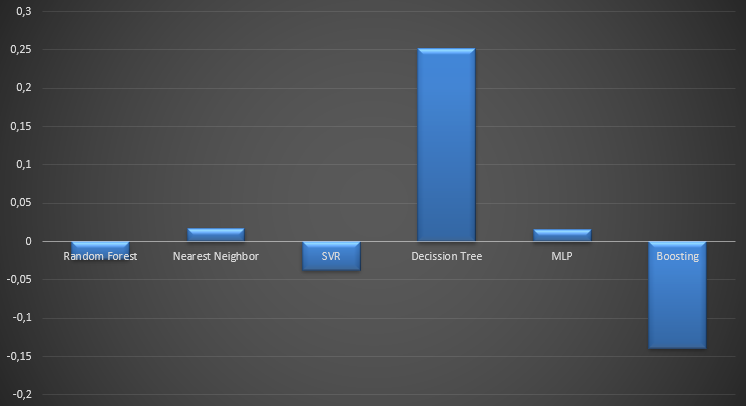
\includegraphics[width=1\textwidth]{grafico_compartiva_modelos.png}
	\caption{Comparativa diferentes modelos}\label{fig:comparativa_modelos}
\end{figure}

En la figura \ref{fig:comparativa_modelos} podemos observar como el modelo que mejores resultados nos aporta, es el de arboles de decisión. Se ha utilizado como parámetro de puntuación el coeficiente de determinación o \(R^2\). Este es una medida de la calidad del ajuste del modelo.

Este modelo nos ha otorgado un coeficiente de determinación de 0,25. Esto nos indica que el modelo no realiza una predicción suficientemente precisa de los avistamientos por lo que habría que realizar un mayor tratamiento de los datos previamente a el entrenamiento del mismo.

Se ha realizado una prueba con la playa que contaba con el mayor número de días con avistamientos. El resultado de la predicción respecto a los datos reales se puede observar en la figura \ref{fig:comparativa}
 
\begin{figure}[!h]
	\centering
	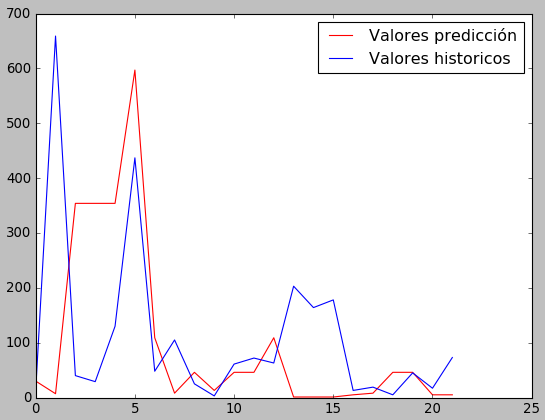
\includegraphics[width=0.8\textwidth]{comparativaModelo.png}
	\caption{Comparativa entre predicción y realidad}\label{fig:comparativa}
\end{figure}